%#################### 7.1 ####################
\subsection{\hll{Simple pie chart}}

\begin{tabular}{c | c}
\begin{minipage}[m]{0.4\textwidth}
\enum{ 
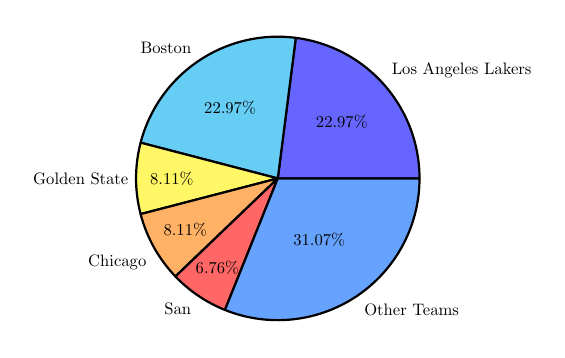
\begin{tikzpicture}[thick,scale=0.6, every node/.style={transform shape}] 
\pie{22.97/Los Angeles Lakers,
22.97/Boston,
8.11/Golden State,
8.11/Chicago,
6.76/San ,
31.07/Other Teams}
\end{tikzpicture}}{\thesubsection}
\end{minipage}
&
\begin{minipage}[m]{0.55\textwidth}
\renewcommand\textminus{\mbox{-}}%<<<<<<<<<<<
\begin{lstlisting}[numberstyle=\zebra{red!15}{yellow!15},numbers=left,basicstyle=\ttfamily\footnotesize]{tex}
\documentclass[border=0.2cm]{standalone} 
\usepackage{pgf-pie}  

\begin{document}
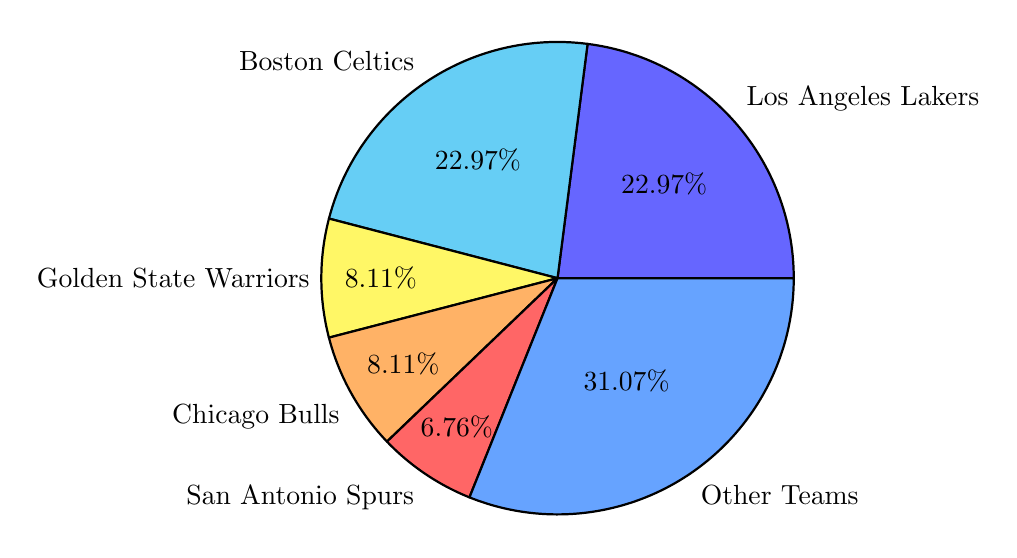
\begin{tikzpicture}
\pie{22.97/Los Angeles Lakers,
22.97/Boston Celtics,
8.11/Golden State Warriors,
8.11/Chicago Bulls,
6.76/San Antonio Spurs,
31.07/Other Teams}
\end{tikzpicture}
\end{document}
\end{lstlisting}
\end{minipage}
\end{tabular}


	%#################### 7.2 ####################
\subsection{\hll{Circled arrows with text}}

\begin{tabular}{c | c}
\begin{minipage}[m]{0.4\textwidth}
\enum{ 
\begin{center}
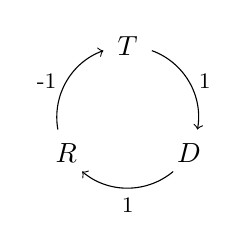
\begin{tikzpicture}[->,scale=.9]
\node (i) at (90:1cm)  {$T$};
\node (j) at (-30:1cm) {$D$};
\node (k) at (210:1cm) {$R$};
\draw (70:1cm)  arc (70:-10:1cm) node[midway, right] {{\footnotesize 1}};
\draw (-50:1cm) arc (-50:-130:1cm) node[midway, below] {{\footnotesize 1}};
\draw (190:1cm) arc (190:110:1cm) node[midway, left] {{\footnotesize -1}};
\end{tikzpicture}\end{center}}{\thesubsection}
\end{minipage}
&
\begin{minipage}[m]{0.55\textwidth}
\renewcommand\textminus{\mbox{-}}%<<<<<<<<<<<
\begin{lstlisting}[numberstyle=\zebra{red!15}{yellow!15},numbers=left,basicstyle=\ttfamily\scriptsize]{tex}
\documentclass{article} 
\usepackage{tikz}

\begin{document}
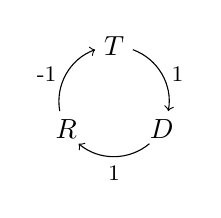
\begin{tikzpicture}[->,scale=.7]
\node (i) at (90:1cm)  {$T$};
\node (j) at (-30:1cm) {$D$};
\node (k) at (210:1cm) {$R$};
\draw (70:1cm)  arc (70:-10:1cm) node[midway, right] {{\footnotesize 1}};
\draw (-50:1cm) arc (-50:-130:1cm) node[midway, below] {{\footnotesize 1}};
\draw (190:1cm) arc (190:110:1cm) node[midway, left] {{\footnotesize -1}};
\end{tikzpicture}
\end{document}
\end{lstlisting}
\end{minipage}
\end{tabular}

\newpage
%#################### 7.3 ####################
\subsection{\hll{Diamond with text}}
	
	\begin{tabular}{c | c}
	\begin{minipage}[m]{0.4\textwidth}
	\enum{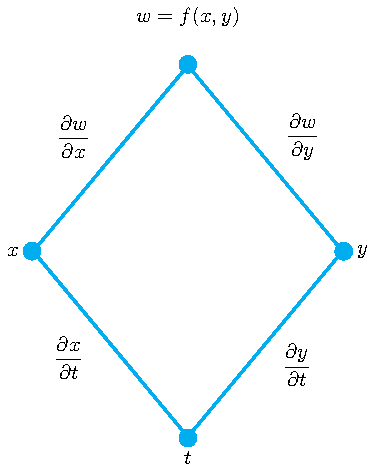
\includegraphics[width=1\linewidth]{7.3.pdf}}{\thesubsection}
	\end{minipage}
	&
	\begin{minipage}[m]{0.55\textwidth}
	\renewcommand\textminus{\mbox{-}}%<<<<<<<<<<<
	\begin{lstlisting}[numberstyle=\zebra{red!15}{yellow!15},numbers=left,basicstyle=\ttfamily\scriptsize]
\documentclass[a4paper,14pt]{extreport}
\usepackage[left=1.5cm,right=1.5cm,top=1.5cm,bottom=2cm,bindingoffset=0cm]{geometry}
\usepackage{amsmath}
\usepackage{tikz}
\usetikzlibrary{shapes.geometric}
 
\begin{document}
\begin{tikzpicture}
\node[diamond,font=\small,
line width=0.4mm,scale=0.7,
    draw = cyan, minimum width = 7.5cm, %text = red,
    minimum height = 9cm] (d) at (0,0) { };
      \node [above=0.5cm] (a) at (d.90) {$w = f(x,y)$};
      \node [above=0.5cm,right=0.1cm] (b) at (d.45) {$\dfrac{\partial w}{\partial y}$};
      \node [above=0.5cm,left=0.1cm] (c) at (d.135) {$\dfrac{\partial w}{\partial x}$};
      \node [left=0.1cm] (dd) at (d.180) {$x$};
      \node [right=0.1cm] (e) at (d.0) {$y$};
      \node [below=0.1cm] (f) at (d.270) {$t$};
      \node [below=0.9cm,right=-0.3cm] (g) at (d.-30) {$\dfrac{\partial y}{\partial t}$};
      \node [below=0.5cm,left=0.1cm] (h) at (d.220) {$\dfrac{\partial x}{\partial t}$};
      \node at (d.90) [cyan,circle,fill,inner sep=3pt]{};
      \node at (d.180) [cyan,circle,fill,inner sep=3pt]{};
      \node at (d.0) [cyan,circle,fill,inner sep=3pt]{};
      \node at (d.270) [cyan,circle,fill,inner sep=3pt]{};
\end{tikzpicture}
\end{document}
\end{lstlisting}
	\end{minipage}
	\end{tabular}
	



%#################### 7.4 ####################
\subsection{\hll{Levels of skills }}

\begin{tabular}{c | c}
\begin{minipage}[m]{0.4\textwidth}
\enum{   
\skills{{Word/1}}\\
\skills{{\LaTeX/6}}\\
\skills{{C++/2}}\\
\skills{{Python/3}}\\
}{\thesubsection}
\end{minipage}
&
\begin{minipage}[m]{0.55\textwidth}
\renewcommand\textminus{\mbox{-}}%<<<<<<<<<<<
\begin{lstlisting}[numberstyle=\zebra{red!15}{yellow!15},numbers=left,basicstyle=\ttfamily\scriptsize]{tex}
\documentclass{report}
\usepackage[T1]{fontenc}
\usepackage{tikz}
\usepackage{xcolor}

\definecolor{white}{RGB}{255,255,255}
\definecolor{gray}{HTML}{4D4D4D}
\definecolor{maingray}{HTML}{B9B9B9}

\newcommand\skills[1]{ 
    \begin{tikzpicture}
        \foreach [count=\i] \x/\y in {#1}{
            \draw[fill=maingray,maingray] (0,\i) rectangle (6,\i+0.4);
            \draw[fill=white,gray](0,\i) rectangle (\y,\i+0.4);
            \node[above right] at (0,\i+0.4) {\x};
        }
    \end{tikzpicture}
}

\begin{document}
\skills{{b/2}}
\skills{{a/1}}
\end{document}
\end{lstlisting}
\end{minipage}
\end{tabular}


%#################### 7.5 ####################
\subsection{\hll{Round levels of skills }}

\begin{tabular}{c | c}
\begin{minipage}[m]{0.4\textwidth}
\enum{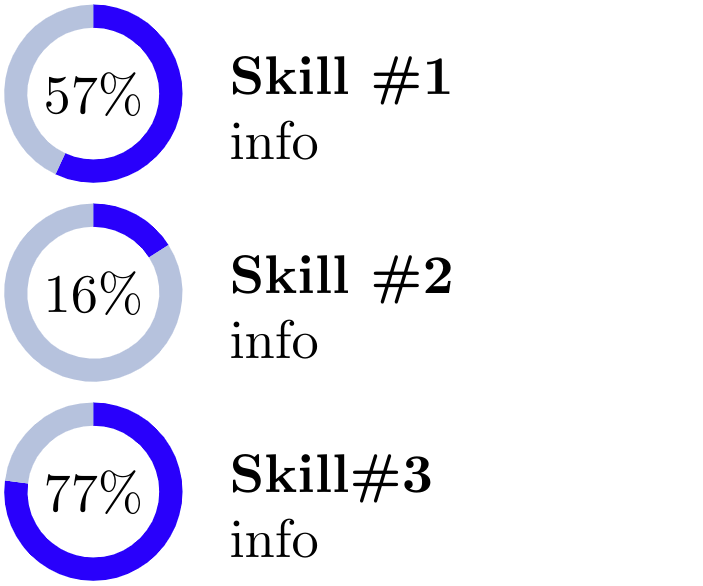
\includegraphics[width=1\linewidth]{7.5.png}}{\thesubsection}
\end{minipage}
&
\begin{minipage}[m]{0.55\textwidth}
\renewcommand\textminus{\mbox{-}}%<<<<<<<<<<<
\begin{lstlisting}[numberstyle=\zebra{red!15}{yellow!15},numbers=left,basicstyle=\ttfamily\scriptsize]{tex}
\documentclass[svgnames]{article}
\usepackage{tikz}
\usetikzlibrary{calc}
\usepackage{siunitx}% only to force percentages to be integers
\usepackage{enumitem}

\let\realItem\item% save for later use
\newcommand\percentageItem[1][10]{%
  \realItem[\smash{\tikz[baseline];
    \draw[thick,line width=1.5mm,Blue](90:5mm)
          arc [radius=5mm, start angle=90, delta angle=-#1*3.6];
    \draw[thick,line width=1.5mm,LightSteelBlue](90-#1*3.6:5mm)
          arc [radius=5mm, start angle=90-#1*3.6, end angle=-270];
    }}]%
}
\newlist{achievements}{itemize}{1}
\setlist[achievements]{
  before=\let\item\percentageItem,%make \item = \percentageItem
  leftmargin=*,
  label={},
  itemsep=3mm,
}

\begin{document}

\begin{achievements}
  \item[57]\textbf{Skill \#1}\\info
  \item[16]\textbf{Skill \#2}\\info
  \item[77]\textbf{Skill \#3}\\info
\end{achievements}

\end{document}
\end{lstlisting}
\end{minipage}
\end{tabular}

%#################### 7.6 ####################
\subsection{\hll{Huge margin line}}

\begin{tabular}{c | c}
\begin{minipage}[m]{0.4\textwidth}
\enum{
\includegraphics[width=0.85\linewidth]{7.6.png}}{\thesubsection}
\end{minipage}
&
\begin{minipage}[m]{0.55\textwidth}
\renewcommand\textminus{\mbox{-}}%<<<<<<<<<<<
\begin{lstlisting}[numberstyle=\zebra{red!15}{yellow!15},numbers=left,basicstyle=\ttfamily\scriptsize]{tex}
\documentclass{article}
\usepackage[margin=3cm]{geometry}
\usepackage{tikz}

\begin{document}
\tikz[overlay, remember picture] \draw[line width=2.5mm] ([xshift=1cm, yshift=-1cm]current page.north west) rectangle ([xshift=-1cm, yshift=1cm]current page.south east);
Text
\vfill
Text
\vfill
Text
\end{document}
\end{lstlisting}
\end{minipage}
\end{tabular}

\newpage
%#################### 7.7 ####################
\subsection{\hll{Aligning anything to a corer}}
\begin{tikzpicture}[remember picture,overlay]
\node[anchor=north east,yshift=0pt,xshift=0pt]%
at (current page.north east)
{\qrcode[height=1.cm]{https://github.com/AnMnv/eBook}% <--- put anything here
};
\end{tikzpicture}

\begin{tabular}{c | c}
\begin{minipage}[m]{0.4\textwidth}
\enum{\center Find me}{\thesubsection}
\end{minipage}
&
\begin{minipage}[m]{0.55\textwidth}
\renewcommand\textminus{\mbox{-}}%<<<<<<<<<<<
\begin{lstlisting}[numberstyle=\zebra{red!15}{yellow!15},numbers=left,basicstyle=\scriptsize]
\documentclass[14pt]{extreport}
\usepackage{tikz}
\usepackage{qrcode}

\begin{document}
\begin{tikzpicture}[remember picture,overlay]
\node[anchor=north west,yshift=0pt,xshift=0pt]%
at (current page.north west)
{\qrcode[height=0.5cm]{https://github.com/AnMnv/eBook}% <--- put here anything
};
\end{tikzpicture}
\end{document}

			OR the rainbow variant (see example 9.7)

\begin{tikzpicture}[remember picture,overlay]
\node at ($(current page.north west)+(.70cm,-.75cm)$) 
    {\fadingtext[scale=0.5]{path picture shading=rainbow}
    {\qrcode[height=3cm]{https://github.com/AnMnv/eBook}}};
\end{tikzpicture}
\end{lstlisting}
\end{minipage}
\end{tabular}

%#################### 7.8 ####################
\subsection{\hll{Family tree}}
\begin{tikzpicture}[remember picture,overlay]
\node[anchor=north east,yshift=0pt,xshift=0pt]%
at (current page.north east)
{\qrcode[height=1.cm]{https://github.com/AnMnv/eBook}% <--- put here anything
};
\end{tikzpicture}

\begin{tabular}{c | c}
\begin{minipage}[m]{0.4\textwidth}
\enum{\begin{tikzpicture}[scale=0.5, every node/.style={scale=0.5},level 1/.style={sibling distance=5cm},level 2/.style={sibling distance=2.5cm}]
	\node {My Family Tree}[edge from parent fork down]
		child { node {Uncle  - Aunty }}
		child { node {Mum - Dad}
			child {node{Me}}
			child {node{My sister}}
			}	
		child { node { Tom -  Sue}
			 child {node{ Josh}}
			 child {node{ Sarah}}
			};
\end{tikzpicture}

\vspace{1.0cm}

\begin{tikzpicture}[scale=0.5, every node/.style={scale=0.5},rotate=180,level 1/.style={sibling distance=5cm},level 2/.style={sibling distance=2.5cm}]
	\node {My Family Tree}[edge from parent fork down]
		child { node {Uncle  -  Jane}}
		child { node {Mum - Dad}
			child {node{Me}}
			child {node{sister}}
			}	
		child { node {Uncle  -  Sue}
			 child {node{ Josh}}
			 child {node{ Sarah}}
			};
\end{tikzpicture}}{\thesubsection}
\end{minipage}
&
\begin{minipage}[m]{0.55\textwidth}
\renewcommand\textminus{\mbox{-}}%<<<<<<<<<<<
\begin{lstlisting}[numberstyle=\zebra{red!15}{yellow!15},numbers=left,basicstyle=\ttfamily\scriptsize]
\documentclass{article}
\usepackage{tikz}
\usetikzlibrary{trees}

\begin{document}
\begin{tikzpicture}[level 1/.style={sibling distance=5cm},level 2/.style={sibling distance=2.5cm}]
	\node {My Family Tree}[edge from parent fork down]
		child { node {Uncle John - Aunty Jane}}
		child { node {Mum - Dad}
			child {node{Me}}
			child {node{My sister}}
			}	
		child { node {Uncle Tom - Aunty Sue}
			 child {node{Cousin Josh}}
			 child {node{Cousin Sarah}}
			};
\end{tikzpicture}
\end{document}
\end{lstlisting}
\end{minipage}
\end{tabular}

%#################### 7.9 ####################
\begin{landscape}
\subsection{\hll{Mind map}}

\begin{tabular}{c | c}
\begin{minipage}[m]{0.59\textwidth}
\enum{\begin{tikzpicture}[scale=0.7, every node/.style={scale=0.6}]
  \path[mindmap,concept color=black,text=white]
    node[concept] {Computer Science}
    [clockwise from=0]

    child[concept color=green!50!black] {
      node[concept] {qqq}
      [clockwise from=90]
      child { node[concept] {qqq1} }
      child { node[concept] {qqq2} }
      child { node[concept] {qqq3} }
      child { node[concept] {qqq4} }
    }

    child[concept color=blue] {
      node[concept] {ccc}
      [clockwise from=-30]
      child { node[concept] {ccc1} }
      child { node[concept] {ccc2} }
    }
    child[concept color=red] { node[concept] {aaa1} }
    child[concept color=orange] { node[concept] {bbb1} };
\end{tikzpicture}}{\thesubsection}
\end{minipage}
&
\begin{minipage}[m]{0.5\textwidth}
\renewcommand\textminus{\mbox{-}}%<<<<<<<<<<<
\begin{lstlisting}[numberstyle=\zebra{red!15}{yellow!15},numbers=left,basicstyle=\ttfamily\scriptsize]
\documentclass{article}
\usepackage[utf8]{inputenc}
\usepackage{tikz}
\usetikzlibrary{mindmap}
\usetikzlibrary[mindmap]

\begin{document}

\begin{tikzpicture}
  \path[mindmap,concept color=black,text=white]
    node[concept] {Computer Science}
    [clockwise from=0]
    % note that `sibling angle' can only be defined in
    % `level 1 concept/.append style={}'
    child[concept color=green!50!black] {
      node[concept] {practical}
      [clockwise from=90]
      child { node[concept] {algorithms} }
      child { node[concept] {data structures} }
      child { node[concept] {pro\-gramming languages} }
      child { node[concept] {software engineer\-ing} }
    }
    % note that the `concept color' is passed to the `child'(!)
    child[concept color=blue] {
      node[concept] {applied}
      [clockwise from=-30]
      child { node[concept] {databases} }
      child { node[concept] {WWW} }
    }
    child[concept color=red] { node[concept] {technical} }
    child[concept color=orange] { node[concept] {theoretical} };
\end{tikzpicture}

\end{document}
\end{lstlisting}
\end{minipage}
\end{tabular}

\end{landscape}
%#################### 7.10 ####################
\subsection{\hll{Gantt chart}}

\begin{tabular}{c | c}
\begin{minipage}[m]{0.4\textwidth}
\enum{\begin{tikzpicture}[scale=0.8, every node/.style={scale=0.8}]
\tikzset{
    simple gantt/.cd,
    width unit=0.33cm,
    box/.style={draw},
}
\pic at (0,0) {simple gantt={$P_1$/2, $P_2$/3, $P_3$/11, $P_4$/15, $P_5$/20}};


\tikzset{
    simple gantt/.cd,
    height=0.75cm,
    color cycle={yellow, orange, cyan, magenta},
    label pin angle={270},
    label pin/.append style={below},
    tick position={above},
    tick label/.append style={above},
    label as pin if value below={4},
}
\pic at (0,-3) {simple gantt={A/1, B/3, C/9, D/10, E/20, F/25}};
\end{tikzpicture}}{\thesubsection}
\end{minipage}
&
\begin{minipage}[m]{0.55\textwidth}
\renewcommand\textminus{\mbox{-}}%<<<<<<<<<<<
\begin{lstlisting}[numberstyle=\zebra{red!15}{yellow!15},numbers=left,basicstyle=\ttfamily\tiny]
\documentclass[border=10pt]{standalone}
\usepackage{tikz}

\newif\ifsimplegantttickpositionbelow
\tikzset{
pics/simple gantt/.style={
code={
\ifsimplegantttickpositionbelow
\path[/tikz/simple gantt/tick] (0,0) -- 
++(0,{-1*\pgfkeysvalueof{/tikz/simple gantt/tick length}}) 
node[/tikz/simple gantt/tick label] {\pgfmathprintnumber{0}};
\else
\path[/tikz/simple gantt/tick] (0,\pgfkeysvalueof{/tikz/simple gantt/height}) -- 
++(0,{\pgfkeysvalueof{/tikz/simple gantt/tick length}}) 
node[/tikz/simple gantt/tick label] {\pgfmathprintnumber{0}};
\fi
\foreach \n/\x [count=\i, remember=\x as \lastx (initially 0)] in {#1} {
\ifsimplegantttickpositionbelow
\path[/tikz/simple gantt/tick] ({\x*\pgfkeysvalueof{/tikz/simple gantt/width unit}},0) -- 
    ++(0,{-1*\pgfkeysvalueof{/tikz/simple gantt/tick length}}) 
    node[/tikz/simple gantt/tick label] {\pgfmathprintnumber{\x}};
\else
\path[/tikz/simple gantt/tick] ({\x*\pgfkeysvalueof{/tikz/simple gantt/width unit}},\pgfkeysvalueof{/tikz/simple gantt/height}) -- 
    ++(0,{\pgfkeysvalueof{/tikz/simple gantt/tick length}}) 
    node[/tikz/simple gantt/tick label] {\pgfmathprintnumber{\x}};
\fi
\pgfmathparse{int(mod(\i - 1, \pgfkeysvalueof{/tikz/simple gantt/color cycle length}) + 1)} 
\global\pgfkeyslet{/tikz/simple gantt/color cycle step}{\pgfmathresult}
\path[
/tikz/simple gantt/box, 
fill={simple gantt color \pgfkeysvalueof{/tikz/simple gantt/color cycle step}},
]
({\lastx*\pgfkeysvalueof{/tikz/simple gantt/width unit}},0) rectangle 
({\x*\pgfkeysvalueof{/tikz/simple gantt/width unit}},\pgfkeysvalueof{/tikz/simple gantt/height})
\pgfextra{\pgfmathparse{\x - \lastx}}
\ifdim\pgfmathresult pt < \pgfkeysvalueof{/tikz/simple gantt/label as pin if value below} pt\relax
    node[/tikz/simple gantt/label, pin={[/tikz/simple gantt/label pin]\pgfkeysvalueof{/tikz/simple gantt/label pin angle}:\n}] {}
\else
    node[/tikz/simple gantt/label] {\n}
\fi ;}}},
simple gantt/color cycle length/.initial={0},
simple gantt/color cycle step/.initial={1},
simple gantt/color cycle/.code={
\foreach \c [count=\i] in {#1} {
\xglobal\colorlet{simple gantt color \i}{\c}
\global\pgfkeyslet{/tikz/simple gantt/color cycle length}{\i}}},
simple gantt/height/.initial={1cm},
simple gantt/width unit/.initial={1cm},
simple gantt/box/.style={},
simple gantt/label/.style={pos=0.5},
simple gantt/label pin/.style={above, pin edge={black, thin}, pin distance=0.5cm},
simple gantt/label pin angle/.initial={90},
simple gantt/label as pin if value below/.initial={1.5},
simple gantt/tick/.style={draw},
simple gantt/tick label/.style={below},
simple gantt/tick position/.is choice,
simple gantt/tick position/above/.code={\simplegantttickpositionbelowfalse},
simple gantt/tick position/below/.code={\simplegantttickpositionbelowtrue},
simple gantt/tick position={below},
simple gantt/tick length/.initial={5pt},
simple gantt/color cycle={blue!50, red!50, green!50},}

\begin{document}
\begin{tikzpicture}
\tikzset{simple gantt/.cd, width unit=0.33cm,box/.style={draw}}
\pic at (0,0) {simple gantt={$P_1$/2, $P_2$/3, $P_3$/11, $P_4$/15, $P_5$/20}};

\tikzset{simple gantt/.cd, height=0.75cm, color cycle={yellow, orange, cyan, magenta},
label pin angle={270}, label pin/.append style={below}, tick position={above},
tick label/.append style={above},label as pin if value below={4}}
\pic at (0,-3) {simple gantt={A/1, B/3, C/9, D/10, E/20, F/25}};
\end{tikzpicture}
\end{document}
\end{lstlisting}
\end{minipage}
\end{tabular}

%#################### 7.11 ####################
\subsection{\hll{Drawing a stacked venn diagram}}

\begin{tabular}{c | c}
\begin{minipage}[m]{0.4\textwidth}
\enum{
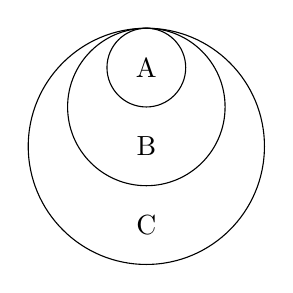
\begin{tikzpicture}[scale=0.5]
\foreach \x [count=\y] in {A,B,C} {
    \draw (0,{-\y}) circle[radius=\y];
    \node at (0,{-2*\y+1}) {\x};
} 
\end{tikzpicture}
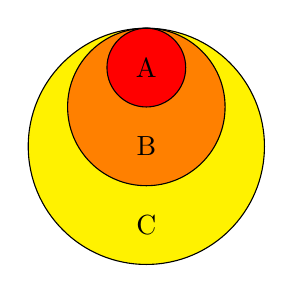
\begin{tikzpicture}[scale=0.5]
\foreach \x/\z [count=\y] in {C/yellow,B/orange,A/red} {
    \draw[fill=\z] (0,{\y-4}) circle[radius={4-\y}];
    \node at (0,{-2*(4-\y)+1}) {\x};
} 
\end{tikzpicture}}{\thesubsection}
\end{minipage}
&
\begin{minipage}[m]{0.55\textwidth}
\renewcommand\textminus{\mbox{-}}%<<<<<<<<<<<
\begin{lstlisting}[numberstyle=\zebra{red!15}{yellow!15},numbers=left,basicstyle=\scriptsize]
\documentclass[border=10pt]{standalone}
\usepackage{tikz}

\begin{document}
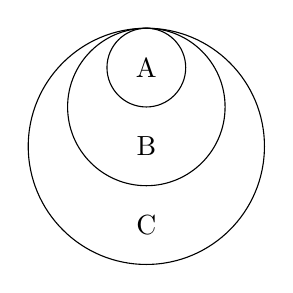
\begin{tikzpicture}[scale=0.5]
\foreach \x [count=\y] in {A,B,C} {
    \draw (0,{-\y}) circle[radius=\y];
    \node at (0,{-2*\y+1}) {\x};
} 
\end{tikzpicture}
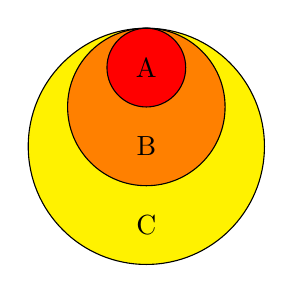
\begin{tikzpicture}[scale=0.5]
\foreach \x/\z [count=\y] in {C/yellow,B/orange,A/red} {
    \draw[fill=\z] (0,{\y-4}) circle[radius={4-\y}];
    \node at (0,{-2*(4-\y)+1}) {\x};
} 
\end{tikzpicture}
\end{document}
\end{lstlisting}
\end{minipage}
\end{tabular}

%#################### 7.12 ####################
\begin{landscape}
\subsection{\hll{Ellipsis in Circuitikz}}
%https://tex.stackexchange.com/questions/232924/ellipsis-in-circuitikz

\begin{tabular}{c | c}
\begin{minipage}[m]{0.65\textwidth}
\enum{
\begin{circuitikz}[line width=1pt]
  \draw (0,2) to[L,l=$L'$,*-*] (2,2)
        (2,0) to[C,l=$C'$,-*] (2,2)
        (2,0) to[short,-*] (0,0)
  ;
  \begin{scope}[xshift=2cm]
  \draw (0,2) to[L,l=$L'$,*-*] (2,2)
        (2,0) to[C,l=$C'$,-*] (2,2)
        (2,0) to[short,-*] (0,0)
  ;
  \end{scope}
  \begin{scope}[xshift=4cm]
  \draw (0,2) to[L,l=$L'$,*-*] (2,2)
        (2,0) to[C,l=$C'$,-*] (2,2)
        (2,0) to[short,-*] (0,0)
  ;
  \end{scope}
  \begin{scope}[xshift=6cm]
  \draw (0,2) --  (2,2)node[midway,scale=2,fill=white]{$\cdots$};
  \draw (0,0) -- (2,0)node[midway,scale=2,fill=white]{$\cdots$};
  \end{scope}
  \draw (8,2) to[L,l=$L'$,-*] (10,2) to[short,-*] (11,2)
        (10,0) to[C,l=$C'$,-*] (10,2)
        (11,0) to[short,*-](10,0) to[short,*-] (8,0)
  ;
\end{circuitikz}}{\thesubsection}
\end{minipage}
&
\begin{minipage}[m]{0.5\textwidth}
\renewcommand\textminus{\mbox{-}}%<<<<<<<<<<<
\begin{lstlisting}[numberstyle=\zebra{red!15}{yellow!15},numbers=left,basicstyle=\scriptsize]
\documentclass{article}
\usepackage{circuitikz}
\ctikzset{bipoles/thickness =1}
\begin{document}
\begin{circuitikz}[line width=1pt]
  \draw (0,2) to[L,l=$L'$,*-*] (2,2)
        (2,0) to[C,l=$C'$,-*] (2,2)
        (2,0) to[short,-*] (0,0)
  ;
  \begin{scope}[xshift=2cm]
  \draw (0,2) to[L,l=$L'$,*-*] (2,2)
        (2,0) to[C,l=$C'$,-*] (2,2)
        (2,0) to[short,-*] (0,0)
  ;
  \end{scope}
  \begin{scope}[xshift=4cm]
  \draw (0,2) to[L,l=$L'$,*-*] (2,2)
        (2,0) to[C,l=$C'$,-*] (2,2)
        (2,0) to[short,-*] (0,0)
  ;
  \end{scope}
  \begin{scope}[xshift=6cm]
  \draw (0,2) --  (2,2)node[midway,scale=2,fill=white]{$\cdots$};
  \draw (0,0) -- (2,0)node[midway,scale=2,fill=white]{$\cdots$};
  \end{scope}
  \draw (8,2) to[L,l=$L'$,-*] (10,2) to[short,-*] (11,2)
        (10,0) to[C,l=$C'$,-*] (10,2)
        (11,0) to[short,*-](10,0) to[short,*-] (8,0)
  ;
\end{circuitikz}
\end{document}
\end{lstlisting}
\end{minipage}
\end{tabular}

\end{landscape}
%#################### 7.13 ####################
%#################### 7.14 ####################
%#################### 7.15 ####################
%#################### 7.16 ####################
%#################### 7.17 ####################













